\begin{frame}
    \frametitle{Lemma 1 - Brodcast Conformity}
    \begin{lemma}
        If a correct process $p_i$ recives a message $m$ from a $r\_brodcast(m)$ by another correct process - 
        any other correct process will recive $m$.\\
    \end{lemma}

    \begin{proof}
        Immidiate from the guarantees of the broadcast algorithm.
    \end{proof}
\end{frame}
\begin{frame}
    \frametitle{Lemma 2 - Correct Process Intersection}
    \begin{lemma}
        Any two sets of processes of size $(n-t)$ must have
        at least one correct process in common.
    \end{lemma}
    \begin{center}
        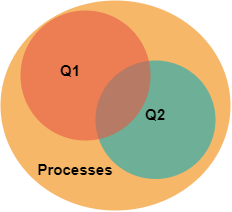
\includegraphics[scale=.5]{lemma2_venn.png}
    \end{center}
\end{frame}
\begin{frame}
    \frametitle{Lemma 2 - Correct Process Intersection. Proof.}
    \begin{proof}
        Denote the set of processes with $P$, and the set of faulty ones $F$.\\
        Let $Q_1,Q_2\subseteq P$ s.t. $|Q_1|=|Q_2|=n-t$.\\
        \[
            |\overline{Q}_1\cup\overline{Q}_2|\leq |\overline{Q}_1|+|\overline{Q}_2|
            \Rightarrow n-|\overline{Q}_1\cup\overline{Q}_2|\geq n-|\overline{Q}_1|-|\overline{Q}_2|
        \]\[
            \Rightarrow |\overline{\overline{Q}_1\cup\overline{Q}_2}|\geq n-t-t
        \]\[
            \Rightarrow |Q_1\cap Q_2|\geq n-2t>3t-2t=t=|F|
        \]\[
            \Rightarrow \exists p\in Q_1\cap Q_2\notin F
        \]
    \end{proof}
\end{frame}

\subsection{Termination Properties}
\begin{frame}
    \frametitle{Lemma 3 - Write Termination}
    \begin{lemma}
        Let $p_i$ be a correct process.
        Any invocation of $Reg[i].write()$ terminates.
    \end{lemma}
    \begin{proof}
        By induction; Assume $k$'th write invocation by $p_i$ recives $WRTIE\_DONE$ from all correct processes.
        \begin{itemize}
            \item When $p_i$ invokes write for $k+1$ time, it brodcasts $WRITE$.
            \item All correct processes recive $WRITE$ (eventually).
            \item In each of those, $reg[j].sn$ is $k$ due to induction assumption (line 12).
            \item (line 12) satisfied and $WRITE\_DONE$ is sent back.
        \end{itemize}
    \end{proof}
\end{frame}
\begin{frame}
    \frametitle{Lemma 4 - Read Termination}
    \begin{lemma}
        Let $p_i$ be a correct process. Any invocation of $Reg_i[j].read()$ terminates.
    \end{lemma}
\end{frame}
\setbeamertemplate{itemize items}[circle]
\begin{frame}{Lemma 4 - Read Termination. Proof.}
    Druring the read, $p_i$ brodcasts $READ(j,rsn)$ where $rsn$ is a sequence number 
    unique to this read. Due to reliable brodcast, $n-t$ correct processes recive and handle
    it eventually and sends a value $wsn_k$. Now cosider that $p_k$ (a correct process)
    has sent $wsn_k=Reg_k[j].sn$, meaning at some point it must have recived a
    reliable brodcast message $WRITE(\_,wsn_k)$, due to lemma 1 - this means $p_i$ will
    eventually recive $WRITE(\_,wsn_k)$ too. At that point, $Reg_i[j].sn$ will also
    be at-least $wsn_k$.\\
    So eventually - there are $n-t$ correct processes sending $STATE(\_, wsn_k)$
    and for each $Reg_i[j]\geq wsn_k$ eventually. This means line (7) will finish at some point.\\
\end{frame}
\begin{frame}
    \frametitle{Lemma 4 - Read Termination. Proof.}
    The next possible stall to the \emph{read} invocation is at line (10) -
    \emph{'wait $CATCH\_UP\_DONE(j,x)$' from $n-t$ different processes}.\\
    At line (9) we brodcast $CATCH\_UP(j,x)$, so all correct processes
    eventually recive it. Consider $p_k$ which has recived $CATCH\_UP(j,x)$;
    for $p_i$ to have arrived when $Reg_i[j].sn=x$, all $WRITE$ messages 
    of the first $x$ writes by $p_j$ must have arrived at $p_i$, due to reliable
    brodcast - all these messages must arrive at $p_k$ too. When the last of them does - 
    $Reg_k[j].sn$ is at-least $x$ causing the wait at line (16) to terminate thus
    $p_k$ sends $CATCH\_UP\_DONE(j,x)$ to $p_i$.\\
    When the last process $p_k$ sends $CATCH\_UP\_DONE$ - $p_i$ can terminate.
\end{frame}

\subsection{Atomicity Properties (Write History Sequence)}
\begin{frame}
    \frametitle{Lemma 5 - Write Serialization}
    \begin{lemma}
        It is possible to associate a single sequence of values $H_i$
        with each register $Reg[i]$. Moreover, if $p_i$ is correct -
        $H_i$ is the sequence of values written to $Reg[i]$ by $p_i$.
    \end{lemma}
\end{frame}
\begin{frame}
    \frametitle{Lemma 6 - Read before Write}
    \begin{lemma}
        Let $p_i, p_j$ be two correct processes.\\
        If $read[i,j,x]$ terminates before $write[j,y]$ starts, then $x<y$.
    \end{lemma}
\end{frame}
\begin{frame}
    \frametitle{Lemma 6 - Read before Write. Proof.}
        Let $read[i,j,x]$ terminate before $write[j,y]$ starts.\\
        During the execution of $read[i,j,x]$ at line (8), the value of $read[i,j,x]$
        is $x$ (by def.).\\
        Additionally - during the write, $p_j$ sends $WRITE$ to
        $p_i$, denote the value of $reg_i[j]$ at the time of it's arrival
        with $r$. Now note how $y=r+1$ due to the condition at (12) (and thanks to termination property).\\
        Also, $x$ and $r$ are both value of $reg_j[i]$ which only increases it's value.
        Piecing it all together gives:
        \[
            x\leq r<r+1=y \Rightarrow x<y
        \]
\end{frame}
\begin{frame}
    \frametitle{Lemma 7 - Write before Read}
    \begin{lemma}
        Let $p_i, p_j$ be two correct processes.\\
        If $write[i,x]$ terminates before $read[j,i,y]$ starts, then $x\leq y$.
    \end{lemma}
\end{frame}
\begin{frame}
    \frametitle{Lemma 7 - Write before Read. Proof.}
    The fact that $write[i,x]$ terminates before $read[j,i,y]$ starts
    implies that at least $n-t$ processes have responded to the
    $WRITE(*,x)$ message sent by $p_i$ at line we (2) - before $read[j,i,y]$ has started. Denote
    this set of processes with \alert{$Q_1$}.\\
    During $read[j,i,y]$, at line (10) - $p_j$ will wait for a $CATCH\_UP\_DONE$ response from
    $n-t$ processes for the message it sent at line (9).
    Denote this set of processes with \alert{$Q_2$}.\\
    Due to lemma 2, there must be at least one correct process s.t. \alert{
        \[p_k\in Q_1\cap Q_2\]
    }.
\end{frame}
\begin{frame}
    \frametitle{Lemma 7 - Write before Read. Proof.}
    This means that $p_k$ is a \alert{correct process} which responded to
    $WRITE(*,x)$ with $WRITE\_DONE(*,x)$ and \alert{later} responded to $CATCH\_UP(j,y)$ with
    $CATCH\_UP\_DONE(j,y)$.\\
    At time $t_{WD}$ of sending $WRITE\_DONE(*,x)$; $Reg_k[j].sn$ was associated
    with $x$, and later at time $t_{CUD}$ when sending $CATCH\_U\_DONE(j,y)$; $Reg_k[j]$ was associated
    with $y$.\\
    Since $Reg_k[j]$ only increases in value:
    \[
        x=Reg_k[j]_{t_{WD}}\leq Reg_k[j]_{t_{CUD}}=y    
    \]
    \[\blacksquare \]
\end{frame}

\begin{frame}
    \frametitle{Lemma 8 - No Read Inversion}
    \begin{lemma}
        Let $p_i, p_j$ be two correct processes.\\
        If $read[i,k,x]$ terminates before $read[j,k,y]$ starts, then $x\leq y$.
    \end{lemma}
\end{frame}
\begin{frame}
    \frametitle{Lemma 8 - No Read Inversion. Proof.}
    Assume $read[i,k,x]$ terminates before $read[j,k,y]$
    begins; similarly to lemma 7,
    consider the set of processes which have responded to
    $CATCH\_UP(k, x)$ from $p_i$ during $read[i,k,x]$; denote it with $Q_1$.\\
    Consider the set of processes which have responded to
    $CATCH\_UP(k,y)$ from $p_j$ during $read[j,k,y]$; denote it with $Q_2$.\\
    Due to lemma 2, there is a correct process $p_k\in Q_1\cap Q_2$.\\
    Once again both $x=Reg_k[j].sn$ and $y=Reg_k[j].sn$ at different times,
    $x$'s time is prior to that of $y$,
    meaning $x\leq y$.
\end{frame}

\subsection{Piecing it all together}
\begin{frame}
    \begin{theorem}
        The algorithm showcased implements and array of $n$ SWMR
        registers with atomic Consistency, in $BAMP$ with $t<\frac{n}{3}$ systems.
    \end{theorem}
    \begin{proof}
        We have seen required termination properties in lemmas 3,4 and atomicity
        properties in lemmas 5,6,7,8.\\
    \end{proof}
\end{frame}

\begin{frame}
    \frametitle{Complexity}
    
    \begin{block}{Read Complexity}
        \alert{$O(n)$} messages are required for each read - as can be seen
        by the brodcasts at lines (6) and (9).
    \end{block}
    \begin{block}{Write Complexity}
        \alert{$O(n^2)$} messages are required for each write,
        since for a \alert{reliable} brodcast is required
        by the write invocation - which could require up to $O(n^2)$
        messages to be sent. 
    \end{block}
\end{frame}